In this chapter explain the basics of interactive rigid body dynamics simulation.

\section{Problem statement}
Interactive physics simulation is a complex and vast problem. 

\section{Definitions}
A \textbf{rigid body }is an idealized solid object which will never change its shape, even under high forces.

A \textbf{mesh} is a 3D object made of vertices, edges and faces. 

A \textbf{convex mesh} is a mesh whose internal angles are all less or equal to $180\degree$.

\section{Principles of rigid body dynamics simulation}
The section is heavily inspired by \cite{bender2014interactive}. The simulation of rigid body dynamics is usually built around the loop presented in \cref{fig:star_simul_loop}. The simulator begins by finding the collision points between objects (Collision detection). These points are used to derive motion laws which are solved to determine the forces that act on the objects and prevent them from inter-penetrating (Contact handling). Newly found contact points imply collisions, which generate infinite impulse forces, which are handled by collision resolution. When all the contact forces have been computed, the position and velocities of the bodies are integrated forward in time before a new iteration starts.

\begin{figure}[htp]
\center
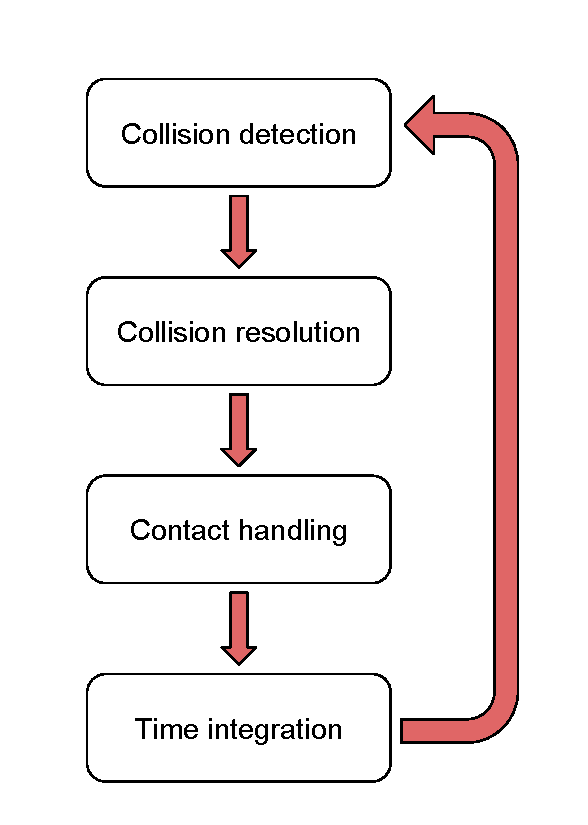
\includegraphics[width=0.3\textwidth]{figures/star_simul_loop2}
\caption[Simulation loop]{Simulation loop}
\label{fig:star_simul_loop}
\end{figure}

